\section{Preliminaries}
Let $\vecs\xi \in \mathbb{R}^N$ describe the generalized state of the system $d$ dimensions, e.g., the robot's joint positions or the Cartesian space position.
Now let $\vecs f(\vecs \xi)$ be a dynamical system describing the desired velocity at a given state: $\vecs{\dot\xi}^{\mathrm{des}} = \vecs f( \vecs \xi)$.
This DS should be continuous and defined for all states $\vecs \xi$. Furthermore, all trajectories converge to the unique attractor state $\vecs \xi ^a \in \mathbb{R}^N$. 

\subsection{Obstacle Avoidance}
Obstacle avoidance based on Modulation (DSM) for point masses has been proposed in \cite{huber2022avoiding}. A collision-free path is obtained by modulating the initial dynamics $\vect f^I(\vecs \xi)$ as follows:
\begin{equation}
  \vecs f(\vecs \xi) = \textbf{E}(\vecs \xi) \text{diag} \left(\lambda^r, \lambda^e, ..., \lambda^e \right) \textbf{E}(\vecs{\xi})^{-1} \vect f^I(\vecs \xi)
  \label{eq:modulated} 
\end{equation}
where the orthonormal basis matrix $\textbf{E}(\vecs \xi)$, defined as:
\begin{equation}
\textbf{E}(\vecs \xi) = \left[ \textbf{r}(\vecs \xi) \ \textbf{e}_1(\vecs \xi) \ ... \ \textbf{e}_{d-1}(\vecs \xi) \right]
\label{eq:matrix_E}
\end{equation}
with the tangent directions $\textbf{e}_{(\cdot)} \in \mathbb{R}^N$ perpendicular to the surface normal $\vect n(\vecs \xi)$, and $\textbf{r}(\vect{\xi}) =  \left( \vecs{\xi}-\vecs{\xi}^r \right) / \| \vecs \xi-\vecs \xi ^r \|$ is the reference direction, concerning the reference point $\vecs \xi^r \in \mathbb{R}^N$, a point placed inside the obstacle's boundaries.
The eigenvalues in reference direction  $\lambda^r$ and tangent direction $\lambda^e$ are evaluated as follows:
\begin{equation}
\begin{split}
    \lambda^r(\vecs \xi) = 1 - 1 /\Gamma(\vecs \xi) , \quad \lambda^e(\vecs \xi) = 1 + 1 / \Gamma(\vecs \xi)
    \label{eq:eigenvalues}
    \end{split}
\end{equation}
with the continuous distance function $\Gamma(\vecs \xi) \in \mathbb{R}$, which has a value of 1 on the boundary of an obstacle, and $\Gamma(\vecs \xi) > 1$ outside the obstacle (Fig.~\ref{fig:resultant_normal}). In this work, we use following distance function
\begin{equation}
  \Gamma(\vecs \xi) = 1 + \| \vecs \xi - \vecs \xi^b \|  
  \quad \text{with} \quad
  \vecs \xi^b = b (\vecs \xi - \vecs \xi^r) + \vecs \xi^r
  \eqref{eq:distance_function}
\end{equation}
with $b \in \mathbb{R}_{>0}$, such that $\vect \xi^b \in \mathbb{R}^N$ lies on the surface of the obstacle.

As $\lambda^r(\vecs \xi) \leq 1$, the initial dynamics are decreased towards the obstacle, and with $\lambda^e(\vecs \xi) \geq 1$, the dynamics are increased in tangent direction. It has been shown in \cite{huber2022avoiding} that this leads to convergence around (star-shaped) obstacles.

\begin{figure}
\centerline{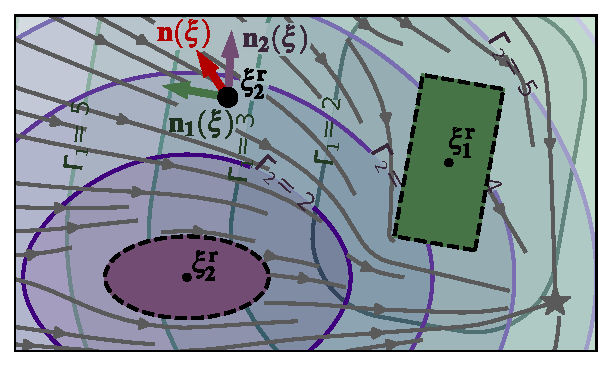
\includegraphics[width=0.5\textwidth]{figures/normal_and_gamma_field_visualization_annotated.pdf}}
\caption{The $\Gamma$-field for the two obstacles is used to evaluate the averaged normal $\vecs n$ (red arrow). 
Both parameters must ensure the motion follows the avoidance dynamics (gray) towards the attractor (black star) while remaining compliant.}
\label{fig:resultant_normal}
\end{figure}

\subsection{Passive Interaction Control} \label{sec:trad_passive}
Passive interaction control \cite{kronander2015passive}is useful for transitioning from velocity-controlled to torque-controlled robots. It allows for selective disturbances rejection, given the direction of motion. For example, one could desire stiff behavior in the direction of the DS but want compliance in the direction perpendicular to the motion.
A stiff behavior means the actual speed will rapidly converge to the desired speed, leading to good tracking performance. Compliance is opposed to stiffness. It is the ability to have flexible behavior and to move away from external forces instead of resisting them.

\begin{definition}[Passivity \cite{willems1972dissipative, sepulchre2012constructive}]
  A dynamical system with input $ u \in \mathcal{U}$ and output $y \in \mathcal{Y}$ is passive with respect to the supply rate $s : \mathcal{U} \times \mathcal{Y} \rightarrow{R}$ if, for any $u: \mathbb{R}_{>0} \rightarrow \mathcal{U}$ and any time $t \geq 0$ the following is satisfied
  \begin{equation}
    \int_0^t s \left( u(\tau),  y (\tau) \right) \geq c^2
  \end{equation}
  where $c \in \mathbb{R}$ depends on the initial conditions.
\end{definition}

Since two passive systems result in a passive system \cite{sepulchre2012constructive}, ensuring that a passive robotic controller is passive will directly ensure that interaction with its (passive) environment results in a passive one.

Both behaviors benefit a robot, and passive control provides a reliable way to apply those to the robot.
Furthermore, the passive control is modular, and damping can increase the damping (e.g., close to dangerous areas) or decrease (e.g., close to humans). Moreover, a passive controller ensures stable behavior between a robot and its environment, which is its significant advantage. Mainly, given any external force,
% the system will always decrease its \textit{storage function}, often modeled as the system's energy
.

The DS $\vecs f(\vecs \xi)$ now returns the desired speed for a given state, but one still needs to convert this information into motor torques the robot understands. Let us introduce the passive interaction control theory in \cite{kronander2015passive}.

\subsection{Rigid Body Dynamics}
For the robot, we consider rigid-body dynamics described with the generalized state variable $\vecs \xi$:
\begin{equation}
\matd{M}(\vecs\xi)\vecs{\ddot\xi} + \matd{C}(\vecs\xi, \vecs{\dot\xi})\vecs{\dot\xi} + \vect g(\vecs\xi) = \vecs{\tau_c} + \vecs{\tau_e}
 \label{eq:robot_dynamics}
\end{equation}
where $\matd M(\vecs\xi)$ is the mass matrix of the robot, $\matd C(\vecs\xi,\vecs{\dot\xi})$ the Coriolis matrix, and  $\vect g(\vecs\xi)$ the gravity vector, $\vecs{\tau_c}$ the control torque and $\vecs{\tau_e}$ the external torque (also referred as disturbance).

The passivity control law proposed in \cite{kronander2015passive} has following form:
%% \begin{equation}
%% \vecs{\tau_c} = \vecs G(\vecs\xi) - \vecs D(\vecs\xi)(\vecs{\dot\xi} -\vecs f(\vecs\xi)) 
%% \label{control_command}
%% \end{equation}

\begin{equation}
	\vecs{\tau_c} = \vect g (\vecs\xi) 
	% + \matd{D}(\vect \xi, \dot{\vect \xi}) \dot{\vect \xi}  
	+ \matd{D}(\vecs\xi) \left(\vecs f(\vecs\xi) - \vecs{\dot\xi} \right) 
\label{eq:control_command}
\end{equation}

This control law embeds a gravity compensation term and a damping term, which decreases the difference between the desired velocity $\vecs f(\vecs\xi)$ and the actual velocity $\vecs{\dot\xi}$.
The damping matrix $\matd D(\vecs\xi)$ is designed to allow for damping in each sub-direction as follows:
%% To have selective damping depending on the direction, one must carefully design  as a matrix composition:
%% \begin{equation}
%% \vecs D(\vecs\xi) = \vecs Q(\vecs\xi)\vecs\Lambda{\vecs Q(\vecs\xi)^{-1}} 
%% \label{D_matrix_shaping}
%% \end{equation}
\begin{equation}
  %% \matd {D}(\vecs \xi) = \matd{Q}(\vecs\xi)\matd{E}{\matd{Q}(\vecs \xi)^{-1}}
  \matd {D}(\vecs \xi) = \matd{Q}(\vecs\xi)\matd{S}(\vecs\xi) \matd{Q} (\vecs \xi)^{-1}
\label{D_matrix_shaping}
\end{equation}
where $\matd Q(\vecs \xi)$ is an othonormal basis matrix and $\matd{S}(\vecs\xi)$ a diagonal matrix consisting of the damping factors. Let $\vecs{q}_1, \vecs q_2, ..., \vecs q_N$ be an orthonormal basis for $\mathbb{R^N}$ with the first vector pointing in the desired direction of motion, i.e., $\vecs q_1 = \dot{\vecs \xi} / \lVert \dot{\vecs \xi} \rVert$, and the remaining vectors from the orthonormal basis.
% Now let $\matd{Q}(\vecs\xi)$ be the matrix whose columns are the vectors $\vecs{e_1},..., \vecs{e_N}$.
% The coefficient $\lambda_1, ..., \lambda_N \geq 0$ on the diagonal of $\vecs\Lambda$ are the damping factors along the corresponding directions given by the vectors $\vecs{q}_1, ..., \vecs{q}_N$.

A common control strategy is to set $\lambda_1$ to a high value so that the speed along the DS direction moves along the desired speed. The stretching in the remaining directions $\lambda_o$ with $o = 2 .. d$ is set lower to allow compliance perpendicular to the motion. 

%% In the case where $\vecs f (\vecs\xi)$ is conservative (i.e. there exists a potential function $V_f(\vecs \xi)$ such that $\vecs f(\vecs\xi) = -\nabla V_f(\vecs\xi)$), the system is proven to be passive. When $\vecs f (\vecs\xi)$ is not conservative, one has to introduce an energy tank and some other control to maintain passivity. 
